%fiber2chip_modelings
\begin{figure}[!ht]
\centering
	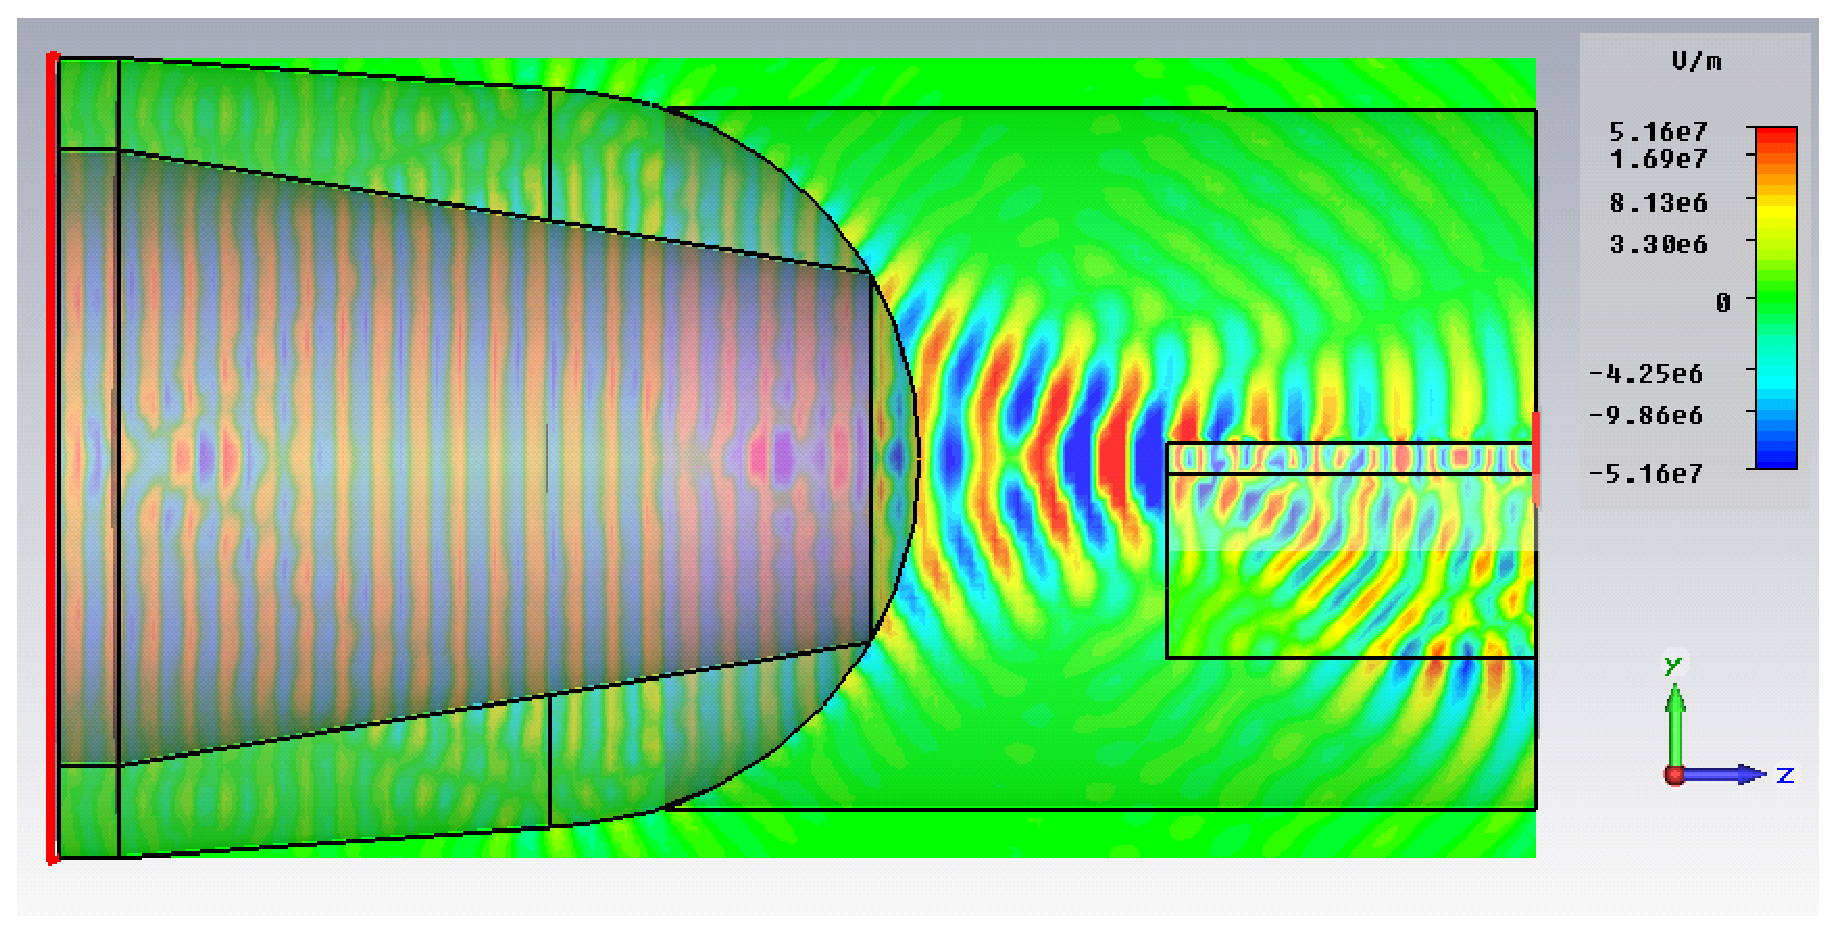
\includegraphics[width=0.7 \textwidth]{bilder/cst_basic_waveguide_efield}
	\caption{E-Field distribution in logarithm value for the Fiber-to-Chip-Interface.}	
	\label{fig:coupling_e_field}
\end{figure}
At the beginning of this chapter the waveguide has been approximated to a rectangular waveguide. To model the coupling interface the waveguide is placed at the distance of $4\mu$m in front of the TLF.  Fig. \ref{fig:coupling_e_field} demonstrate the E-Field distribution of this configuration. It can be seen that the E-Field spreads more widely at the interface of the waveguide than that in the case without the waveguide and a great part of E-Field penetrates into the substrate rather than accepted by guide.\\
 
\begin{figure}[!ht]
\centering
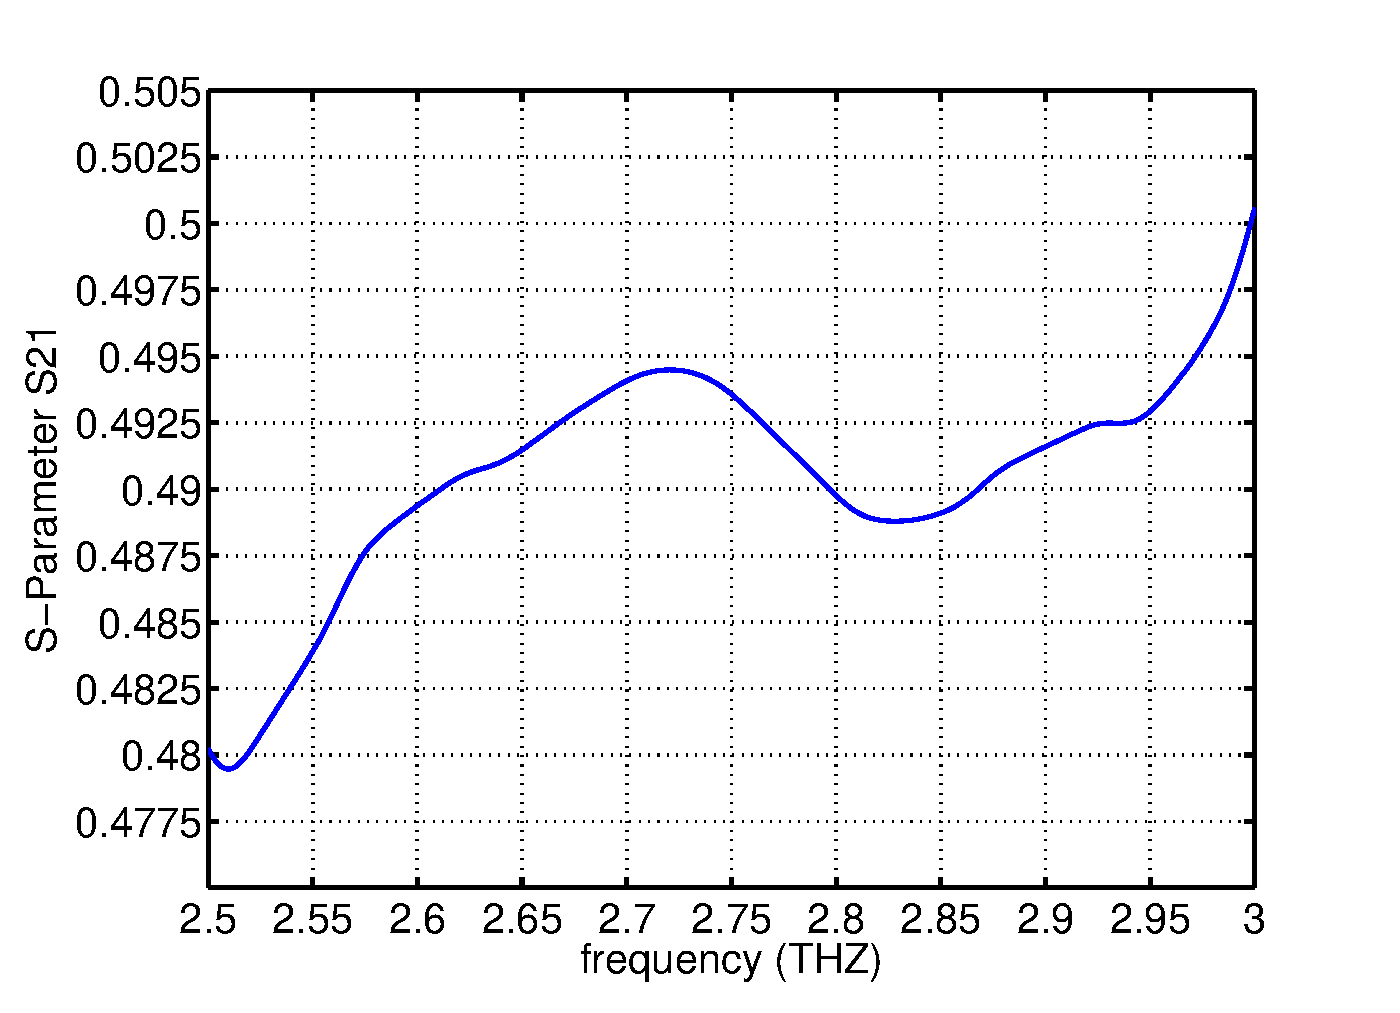
\includegraphics[width=0.7\textwidth]{bilder/original_coupling_efficiency}
\caption{Coupling efficiency in Frequency domain.}
\label{fig:orignial_coupling_efficiency}
\end{figure}
Fig.\ref{fig:orignial_coupling_efficiency} exhibits the coupling efficiency of this configuration in frequency domain. It can be seen that the coupling efficiency at the working frequency $282$THz ($\lambda=1064$nm) is about $48.8\%$. This result will act as the reference sample for the following simulations.\\ 

Furthermore we can analyze the power distribution in this arrangement by executing the integral operation of power flow density over the cross-section of the waveguide (seeing Appendix. \ref{app:powwer_distribution}).  In Fig. \ref{fig:power_distribution} about $40\%$ of the power propagates in the guide while another $40\%$ in the substrate and the rest is losing in the surrounding enviroment or reflected, etc.\\
\begin{figure}[!ht]
\centering
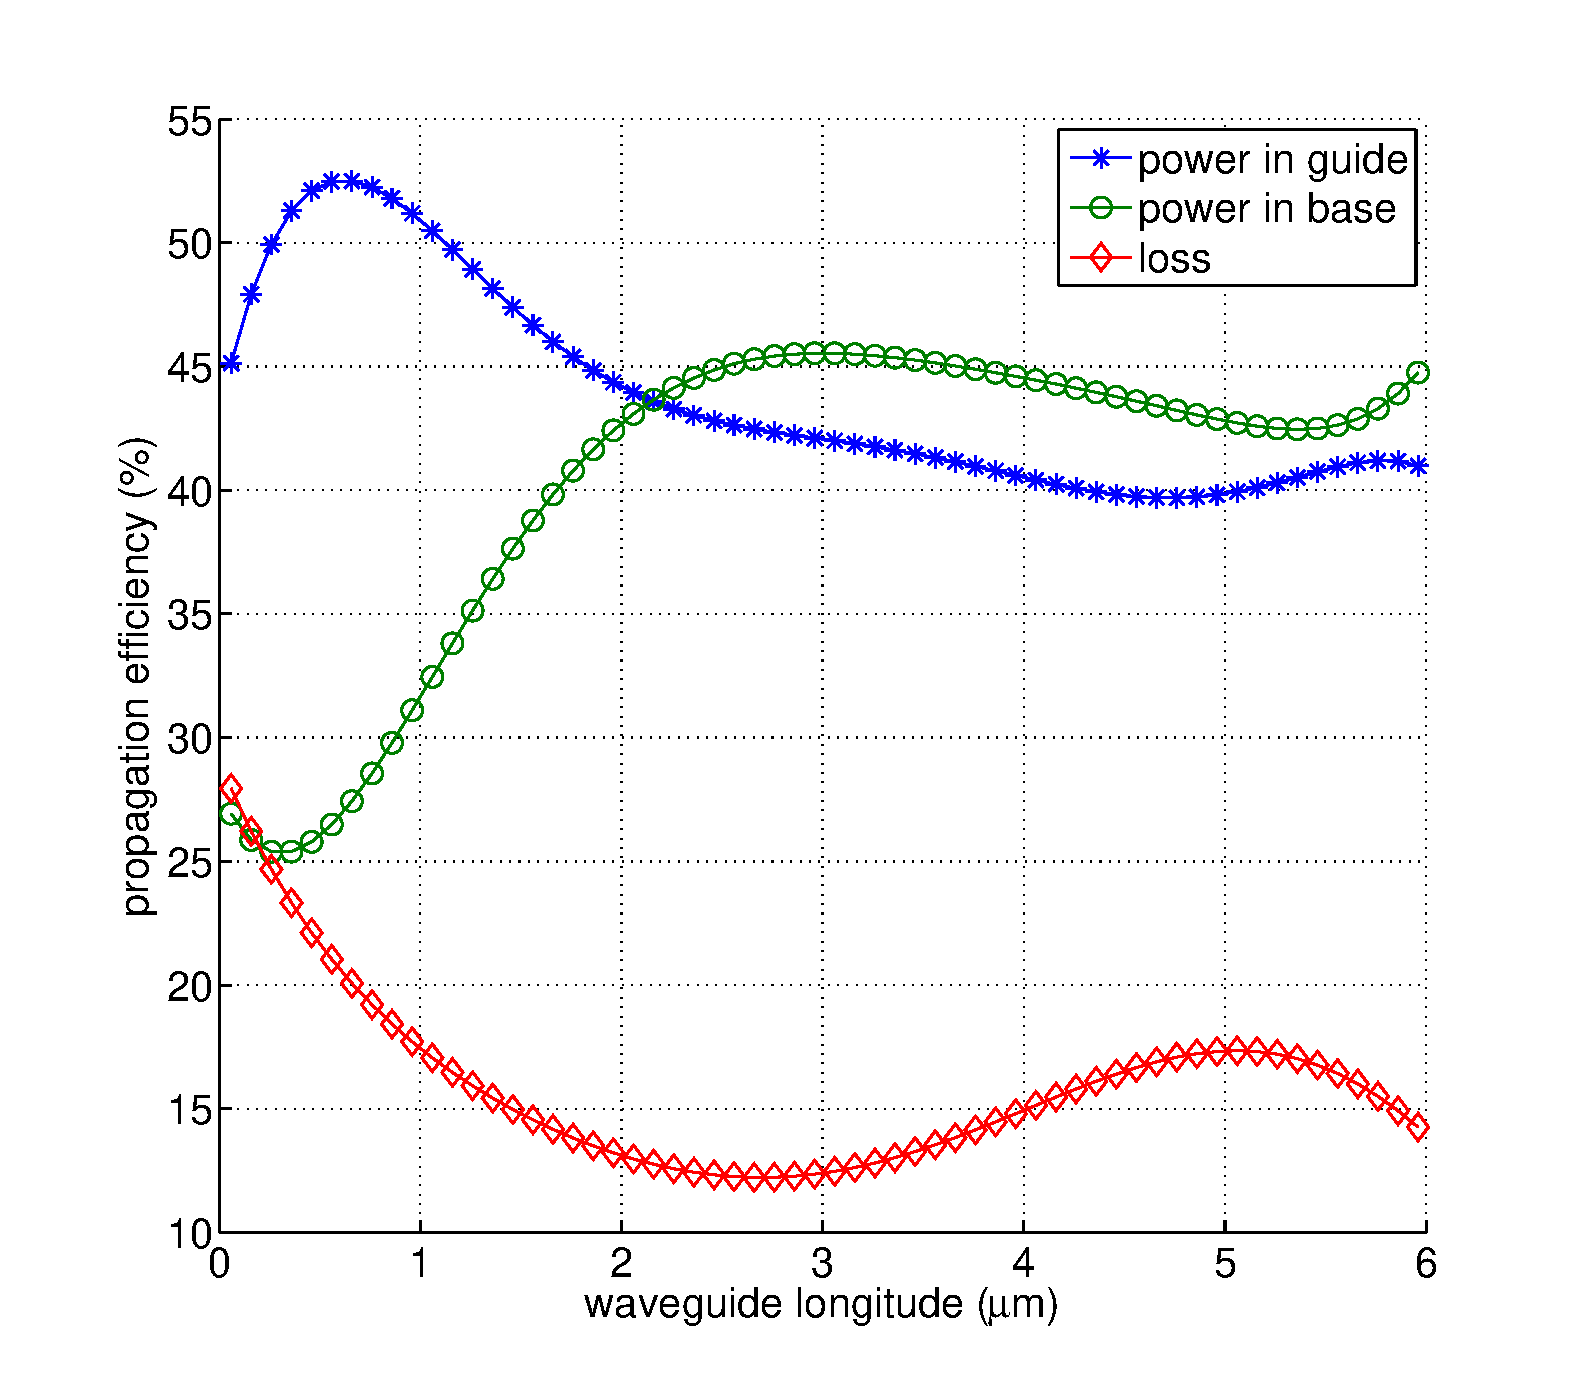
\includegraphics[width=0.7\textwidth]{bilder/power_distribution1}
\caption{Power distribution along the waveguide.}
\label{fig:power_distribution}
\end{figure}
